\documentclass{article}
\usepackage{amsfonts}
\usepackage{amsmath}
\usepackage[margin=2cm]{geometry}
\usepackage{fancybox,color,tcolorbox}
\usepackage{verbatim}
\usepackage[english,spanish,activeacute]{babel}
%\usepackage[latin1]{inputenc}
\usepackage{inputenc}
\usepackage{latexsym}
\usepackage{amsmath}
\usepackage{graphicx} % Allows including images
\usepackage{booktabs}
\usepackage{amssymb}
\usepackage{multimedia}
\usepackage{pifont,pgfcore}
\usepackage{tcolorbox}
\usepackage{animate}
\usepackage{ucs}

\begin{document}

\title{\textbf{Moogle!}}
\author{Dayan Cabrera Corvo}
\date{}

\maketitle

\section* {Descripción}
 Moogle! es una aplicación totalmente original cuyo propósito es buscar inteligentemente un texto en un conjunto de documentos. Es una aplicación web, desarrollada con tecnología .NET Core 6.0, específicamente usando Blazor como framework web para la interfaz gráfica, y en el lenguaje C\#{}. La aplicación está dividida en dos componentes fundamentales: MoogleServer es un servidor web que renderiza la interfaz gráfica y sirve los resultados. MoogleEngine es una biblioteca de clases donde está implementada la lógica del algoritmo de búsqueda.



\vspace{10pt}

\section* {Correr y usar el proyecto}
 Para correr el proyecto debes usar el comandodotnet watch run --project MoogleServer en Windows ymake dev en Linux. En la carpetaContent deberán aparecer los documentos (en formato *.txt) en los que el usuario va a realizar la búsqueda. En la casilla donde aparece Introduzca la búsqueda el usuario va a escribir que desea buscar y basta con apretar el botón Buscar para que Moogle! haga su trabajo.
\vspace{10pt}

\section* {Clase Moogle}
En la clase Moogle convierto la Query en un array de String separándola palabra a palabra y luego la convierto en un vector calculándole su tf, este vector lo multiplico termino a término por el vector que contiene el idf de mis textos y con este vector resultante calculo el score de cada texto multiplicándolo por la matriz donde tengo los TF-IDF de todos mis textos; busco mi Snipet revisando cada texto relevante y buscando la palabra más relevante de ese texto para mi búsqueda y devuelvo 20 palabras antes y después de esta. Por ultimo creo el objeto SearchResoult y lo ordeno según su score con la función Sort de mi clase Ordenar y paso a retornar este objeto.

\vspace{10pt}

\section*{Clase TFIDF}
En primer lugar esta clase accede a los text usando la ruta al contenido.Luego será la encargada de crear un diccionario donde se hacen corresponder las palabras diferentes en todos los txt, con el orden en que van apareciendo. Luego tendría un Lista de arrays(TFIDF) de la siguiente forma, cada posición n de la lista es la posición o valor que se le hace corresponder a la palabra n en el diccionario, de esta forma los arrays serian de tamaño-cantidad de txt. El objetivo de esta Lista es organizar el TFIDF de cada palabra en cada texto. Tenemos una lista (vector\_{}idf) donde se irían guardando los idf de cada palabra. Hay una lista de string (títulos) donde se guardarán los títulos de cada txt. 
\section*{Clase Herramientas}
Aquí tengo dos métodos, uno se encargará de multiplicar una Lista de dobles (donde estará el TFIDF de la query) por la Lista de arrays. El otro hará una multiplicación elemento a elemento de un array y una lista, de iguales dimensiones.
\section*{Clase Levens}
omo la query en caso de que alguna palabra de la query no esté en mis textos la sustituyo por la palabra más similar según la distancia Levenshtein de las que tengo en mis textos , luego devuelvo la cadena resultante como sugestion.
\section*{Funcionalidad de Moogle:}
Cuando el programa se ejecuta, en primer lugar se extraen los txt de la ruta asignada, estos textos se procesan y luego a partir de ellos se calcula el TD, el IDF y el TF-IDF para cada palabra diferente en el documento. Una vez procesada toda esta informacion ya las busquedas saldrian mas rapido. Ahora, las busquedas a su vez son procesadas y llevadas a un array que se ira multiplicando por la (Matriz) con los TFIDF de cada texto, luego se le aplicarian los cambios con respecto a los simbolos y esto nos daria el escore de cada texto. En caso de que una palabra de la busqueda no se encuentre en el conjunto de textos, Moogle le enviara una sugerencia, eso aplica a su vez para palabras mal escritas.
\section*{Simbolos Especiales}
\begin{itemize}
    \item ' !' Delante de una palabra devuelve txt donde esta palabra no puede aparecer.
    \item  '\^{}' Delante de una palabra devuelve txt donde esa palabra tiene que aprecer obligatoriamente
    \item  '\~{}'Entre dos palabras devuelve con mas relevancia los txt donde esas dos palabras aparezcan cerca.
    \item   '*'Se va aumentando el score en dependencia de cuantos aparezcan, para esa o esas palabras
\end{itemize}
\section*{TFIDF Explicacion}
En la descripcion del proyecto se habla sobre los terminos TF e IDF, estos serian: TF: La relacion entre la cantidad de palabras de un documento en especifico(N) y y la cantidad de veces que aparece una palabra en ese documento(n), de la forma: TF=n/N. IDF La relacion entre la cantidad de documentos existentes(D) y la cantidad de documentos que contienen la palabra en cuestion(d): log(1+D/d). De esta forma al realizar la multiplicacion del TF y el IDF, obtendriamos la relvancia de esa palabra en esos documentos.
\section*{Levenshtein Explicacion}
Se trata de un algoritmo de tipo bottom-up, común en programación dinámica. Se apoya en el uso de una matriz (n + 1) × (m + 1), donde n y m son las longitudes de las cadenas. Aquí se indica el algoritmo en pseudocódigo para una función LevenshteinDistance que toma dos cadenas, str1 de longitud lenStr1, y str2 de longitud lenStr2, y calcula la distancia Levenshtein entre ellos.
\begin{figure}[h]
    \centering
	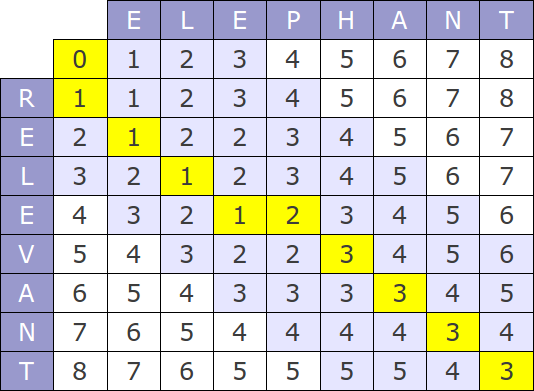
\includegraphics[width=0.68\textwidth]{diagrama.png}
    \caption{Ejemplo de distancia de Lvenshtein}
    \label{img:3}
\end{figure}





\end{document}